\documentclass[conference]{IEEEtran}
\usepackage{graphicx}
\usepackage{amsmath}
\usepackage{caption}
\usepackage{float}

% Title and author
\title{Performance Analysis of Pi Calculation}
\author{Charlie Flux}

\begin{document}
\maketitle

\begin{abstract}
This report examines the performance of the prefix sum algorithm while varying the number of threads and the scalability of these algorithms with a variable array size.
The results show the importance of parallelizable algorithms for speeding up runtimes and that some algorithms are not scalable.
\end{abstract}

\section{Introduction}
The purpose of this experiment is to investigate the impace of multiple threads for execution time on calculating the prefix sum of an array using OpenMP library and the Talapas HPC. 
\section{Methodology}
Three methods for calculating the prefix sum were used:
\begin{itemize}
    \item \textbf{Sliding Window Serial}
    \item \textbf{Sliding Window Parallel} 
    \item \textbf{Binary Tree}
\end{itemize}

For experiments measuring time, core counts \(C\) were chosen from the set:
    \[
    C = \{1, 2, 4, 6, 8, 12, 16, 24, 32, 48, 64, 96, 128\}
    \]
with a fixed dataset size of $65536$. \\
For experiments with variable array size \(N\), where sizes were chosen from the set:
    \[
    N = \{2^1, 2^2, \dots, 2^{16}\} = \{2, 4, 8, 16, 32, \dots, 65536\}
    \]

\subsection{Experimental Setup}
All tests were ran on Talepas. Experiments were repeated 20 times and the average was calculated for each experiment. \\
Data was filtered using the Interquartile Range Filter to remove points that do not lie between the first and third quartile as a consequence of the the unreliable data caused by the unlocked variable frequencies on Telepas.

\section{Results}
\subsection{Critical vs Atomic}
Figure \ref{fig:prefix} has a logarithmic y-axis and compares the execution time of the sliding window and the tree based methods of calculating the prefix sum of an array. 
The graph shows that the sliding window method is not efficient once parallel as the execution time increases as the number of threads increase.
On the other hand the tree based algorithm has a slight performance increase when the number of threads are increased. 
\begin{figure}[H]
    \centering
    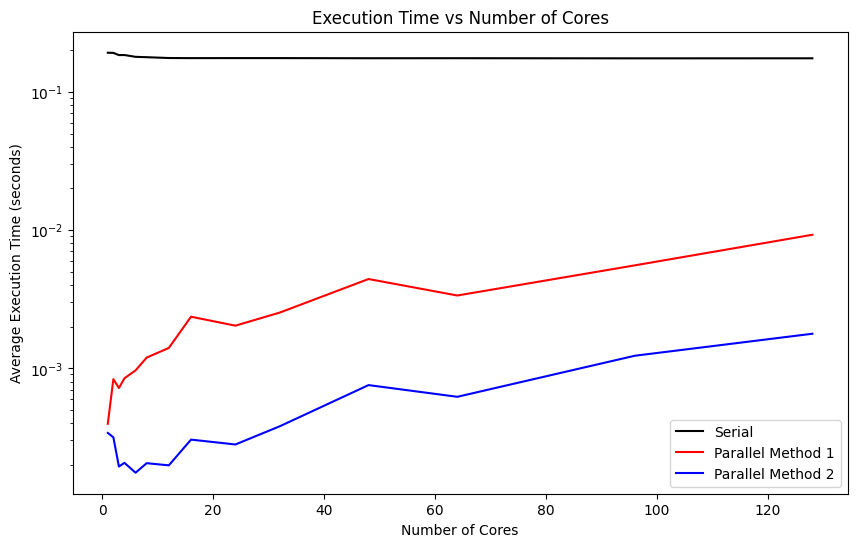
\includegraphics[width=0.45\textwidth]{../img/prefix.png}
    \caption{Sliding Window vs Belloch Scan Execution Time}
    \label{fig:prefix}
\end{figure}

\subsection{Variable Sized Array}
In Figure \ref{fig:variable} I adjusted the size of the array that was worked on while locking the threads used to 32. The binary tree method performed the best due to the parallel nature of the method.
The sliding window method stayed consistent across the range of array sizes which suggests that there is a high overhead or that it is less efficient compared to the binary tree method when parallel.
\begin{figure}[H]
    \centering
    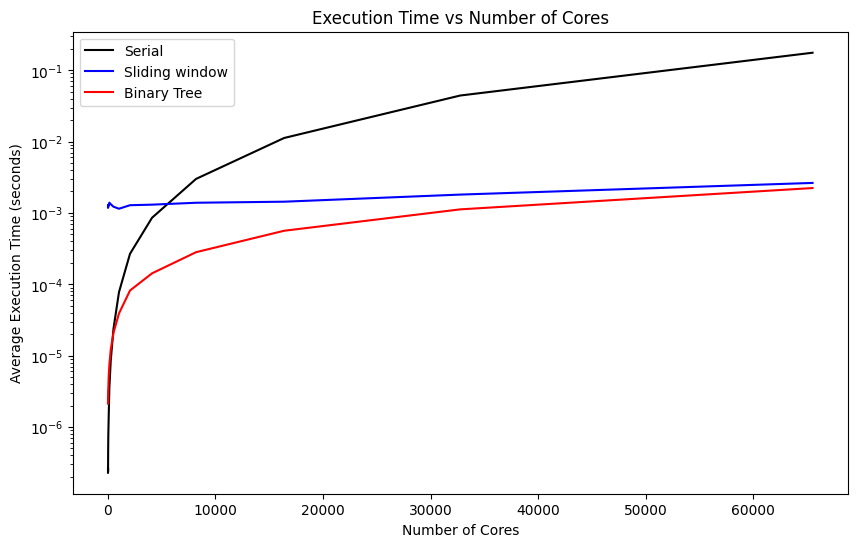
\includegraphics[width=0.45\textwidth]{../img/variable_size.png}
    \caption{Speedup using Reduction}
    \label{fig:variable}
\end{figure}

\section{Conclusion}
The experiments show that the a parallel approach is superior to a serial approach when find this prefix sum of an array. 
The binary tree method showed it was scalable as the performance improved as the thread count increased whereas the sliding window method struggled to scale.
For large scale processing the binary tree method would be superior due to its performance at high thread counts shown in Figure \ref{fig:prefix} and performance at high array sizes shown in Figure \ref{fig:variable}

\end{document}
